\RequirePackage{amsthm}% sn-jnl defines its theorem styles only if amsthm is loaded first
\documentclass[pdflatex,sn-mathphys,Numbered]{sn-jnl}

\usepackage{graphicx}
\usepackage{multirow}
\usepackage{amsmath,amssymb,amsfonts}
\usepackage{amsthm}
\usepackage{xcolor}
\usepackage{booktabs}
\usepackage{algorithm}
\usepackage{algorithmicx}
\usepackage[noend]{algpseudocode}
\usepackage{url}
\usepackage{longtable}
\usepackage{manyfoot}
\usepackage[title]{appendix}
\usepackage{textcomp}

\theoremstyle{thmstyleone}
\newtheorem{theorem}{Theorem}
\newtheorem{lemma}[theorem]{Lemma}
\newtheorem{proposition}[theorem]{Proposition}
\newtheorem{corollary}[theorem]{Corollary}
\theoremstyle{thmstyletwo}
\newtheorem{example}{Example}
\newtheorem{remark}{Remark}
\theoremstyle{thmstylethree}
\newtheorem{definition}{Definition}

\newcommand{\supp}{\operatorname{supp}}
\newcommand{\socc}{\operatorname{occ}}
\newcommand{\Ubo}{\mathrm{UBO}}
\newcommand{\Ucap}{U}
\newcommand{\AURA}{AURA-HOI}
\newcommand{\HEP}{HEP}
\newcommand{\DFHOI}{DFHOI}

% PLACEHOLDER -- overwritten by make_results.py
\newcommand{\MemLimit}{20}
\newcommand{\GeoSpeedupDense}{\textcolor{red}{??}}
\newcommand{\GeoSpeedupSparse}{\textcolor{red}{??}}
\newcommand{\MaxSpeedupDense}{\textcolor{red}{??}}
\newcommand{\NonEmptyConfigs}{\textcolor{red}{??}}
\newcommand{\NumBothFinished}{\textcolor{red}{??}}
\newcommand{\NumConfigs}{\textcolor{red}{??}}
\newcommand{\NumDatasets}{\textcolor{red}{??}}
\newcommand{\NumOracleCases}{\textcolor{red}{??}}
\newcommand{\NumOracleDatabases}{\textcolor{red}{??}}
\newcommand{\OracleMismatches}{\textcolor{red}{??}}
\newcommand{\ParityChecked}{\textcolor{red}{??}}
\newcommand{\ParityMismatches}{\textcolor{red}{??}}
\newcommand{\WinsDFHOI}{\textcolor{red}{??}}

\newcommand{\pending}[1]{\textcolor{red}{[#1]}}
% Primitive \input, so that generated table rows can be included inside tabular environments.
\makeatletter\newcommand{\inputrows}[1]{\@@input #1 }\makeatother

\raggedbottom

\begin{document}

\title[AURA-HOI: Exact High-Occupancy Itemset Mining]{AURA-HOI: High-Occupancy Itemset Mining via Equivalence Classes and Residual Envelope Pruning}

\author*[1]{\fnm{Quan} \sur{Van}}\email{vanhaminhquan2406@gmail.com}

\affil*[1]{\orgname{Independent Researcher}, \orgaddress{\city{Ho Chi Minh City}, \country{Vietnam}}}

\abstract{Occupancy measures how much of its supporting transactions an itemset covers. Because occupancy is not anti-monotone, exact high-occupancy itemset (HOI) miners rely on upper bounds to prune the search space. The bound used by existing miners depends only on the lengths of the supporting transactions; on databases whose transactions all have the same length it degenerates to the support, so these miners must enumerate every frequent itemset. We present AURA-HOI, an exact depth-first miner over prefix equivalence classes of transaction-ID lists. Its central component is a length-capped residual bound that combines transaction lengths with the largest itemset that can still be generated in the current branch. We prove that the bound is safe, that it is never weaker than the transaction-length bound or the purely residual bound, and that the miner returns exactly the set of HOIs. The bound is computed in the same pass as the TID-list intersection, and in constant time when transaction lengths are uniform. We also show that a natural shortcut, taking the residual length from the later siblings only, loses results. In single-threaded experiments on \NumDatasets{} public benchmarks and \NumConfigs{} threshold settings, AURA-HOI returns exactly the same itemsets as two exact baselines, HEP and DFHOI, and agrees with an exact rational-arithmetic oracle on \NumOracleCases{} randomized test cases. It is faster than DFHOI in \WinsDFHOI{} of the \NumBothFinished{} settings, with a geometric-mean speedup of \GeoSpeedupDense{}$\times$ and a maximum of \MaxSpeedupDense{}$\times$ on dense data, where it also performs far fewer candidate intersections. On sparse data its speedup is small (geometric mean \GeoSpeedupSparse{}$\times$).}

\keywords{High-occupancy itemset mining, Pattern mining, Upper bound, Equivalence classes, Vertical mining, Search space pruning}

\maketitle

%%%%%%%%%%%%%%%%%%%%%%%%%%%%%%%%%%%%%%%%%%%%%%%%%%%%%%%%%%%%%%%%%%%%%%%%%%%%%%%%
\section{Introduction}\label{sec:intro}

Frequent itemset mining finds the sets of items that co-occur in at least a given number of transactions \cite{agrawal1993mining,agrawal1994fast}. Its efficient algorithms, such as Apriori \cite{agrawal1994fast}, FP-growth \cite{han2000mining} and Eclat \cite{zaki1997new,zaki2000scalable}, rely on the anti-monotonicity of support: every superset of an infrequent itemset is infrequent. Support alone, however, does not say how representative an itemset is of the transactions that contain it. An itemset of two items that occurs in many transactions of length fifty describes only a small part of each of them.

Tang et al.\ introduced \emph{occupancy} to capture this aspect: the occupancy of an itemset relates its size to the sizes of the transactions that contain it, and patterns with high occupancy are better candidates for recommendation \cite{tang2012occupancy}. Deng formulated the mining of high-occupancy itemsets (HOIs) and proposed the HEP algorithm \cite{deng2020hoi}, and Nguyen et al.\ proposed DFHOI, a depth-first algorithm over equivalence classes with early pruning \cite{nguyen2023dfhoi}. Occupancy has since been studied with transaction weights \cite{datta2022hoimto}, in incremental settings \cite{kim2022incremental}, with adaptive thresholds \cite{tran2025namhep}, as a top-$k$ problem \cite{yildirim2025topk}, and combined with utility \cite{gan2020huopm,kumar2024hauopm,cho2024incremental}.

Occupancy is not anti-monotone: adding an item to an itemset increases its size but may shrink its set of supporting transactions, so the occupancy of the extension can be larger or smaller. Exact miners therefore prune with an \emph{upper bound} on the occupancy of all extensions. The bound used by HEP and DFHOI, which we call the transaction-length bound, exploits the fact that an itemset cannot be larger than any transaction that contains it. It depends only on the lengths of the supporting transactions. When all transactions have the same length, as in many categorical benchmarks, this bound equals the support (Proposition~\ref{prop:uniform}). It then prunes nothing beyond the support constraint, and the miner enumerates every frequent itemset even when none of them has high occupancy.

A depth-first search over prefix equivalence classes provides a second, independent limit: inside a branch, an itemset can only be extended with the items that remain in its class, so its descendants have bounded size. This is the same principle as the remaining-utility bounds of high-utility itemset mining \cite{liu2012huiminer,zida2017efim}. This paper combines the two limits in a single bound and builds an exact miner around it. The main contributions are the following.
\begin{enumerate}
\item A \emph{length-capped residual bound} on the occupancy of every itemset that can still be generated in a branch (Theorem~\ref{thm:capped}). We prove that it is never weaker than the transaction-length bound or the purely residual bound (Proposition~\ref{prop:dominance}), that it is computed in the same linear pass as the TID-list intersection, and that it reduces to a constant-time closed form when transaction lengths are uniform.
\item \AURA{}, a depth-first miner over prefix equivalence classes of TID-lists that applies the bound at the level of nodes and of whole classes and allocates TID-lists from a stack-like arena. We prove that it returns exactly the set of HOIs (Theorem~\ref{thm:correct}), and we show with a two-transaction counterexample that taking the residual length from the later siblings only, a tempting shortcut, loses results (Remark~\ref{rem:pitfall}).
\item An evaluation protocol for exact HOI miners: verification against an exact rational-arithmetic oracle on randomized databases, output parity across algorithms, repeated single-threaded runs without a time limit, memory measured as the increase attributable to the mining phase, an ablation study, a scalability study and a signed-rank test.
\end{enumerate}

Section~\ref{sec:related} reviews related work. Section~\ref{sec:prelim} defines the problem. Section~\ref{sec:bounds} develops the bounds and Section~\ref{sec:algo} the algorithm. Section~\ref{sec:exp} reports the experiments, and Section~\ref{sec:concl} concludes.

%%%%%%%%%%%%%%%%%%%%%%%%%%%%%%%%%%%%%%%%%%%%%%%%%%%%%%%%%%%%%%%%%%%%%%%%%%%%%%%%
\section{Related work}\label{sec:related}

\paragraph{Frequent itemset mining.}
Apriori generates candidates level by level and prunes them with the anti-monotonicity of support \cite{agrawal1993mining,agrawal1994fast}. FP-growth avoids candidate generation by recursively projecting a prefix tree \cite{han2000mining}. Eclat represents each itemset by the sorted list of identifiers of its supporting transactions (its TID-list), groups itemsets that share a prefix into equivalence classes, and computes supports by intersecting TID-lists \cite{zaki1997new,zaki2000scalable}; diffsets reduce the size of these lists on dense data \cite{zaki2003diffsets}. PrePost and PrePost+ use N-lists built from a prefix tree \cite{deng2012nlist,deng2015prepost}. Condensed representations, such as closed \cite{pasquier1999closed,zaki2002charm,uno2004lcm} and maximal \cite{bayardo1998maxminer} itemsets, reduce the number of reported patterns. Surveys of the field are available in \cite{aggarwal2014frequent,fournier2017survey,luna2019review}.

\paragraph{Occupancy.}
Tang et al.\ introduced occupancy as a measure of pattern quality \cite{tang2012occupancy}. Deng studied the mining of high-occupancy itemsets and proposed HEP, which stores occupancy lists and prunes with an upper bound derived from transaction lengths \cite{deng2020hoi}. Nguyen et al.\ proposed DFHOI, which traverses equivalence classes depth-first and applies the bound early \cite{nguyen2023dfhoi}. Datta et al.\ weighted occupancy by transaction occupancy \cite{datta2022hoimto}; Kim et al.\ mined high-occupancy patterns incrementally \cite{kim2022incremental}; Tran et al.\ proposed a hierarchical set-enumeration tree with an adaptive occupancy threshold that changes from level to level \cite{tran2025namhep}; and Y{\i}ld{\i}r{\i}m addressed the top-$k$ problem \cite{yildirim2025topk}. Occupancy has also been combined with utility \cite{gan2020huopm,kumar2024hauopm,cho2024incremental}. The adaptive-threshold and top-$k$ formulations return different result sets from the fixed-threshold problem studied here, so we compare with HEP and DFHOI, which solve the same problem.

\paragraph{Bounds for measures that are not anti-monotone.}
High-utility itemset mining faces the same difficulty, because utility is not anti-monotone either \cite{fournier2019survey,gan2021survey}. HUI-Miner bounds the utility of the extensions of an itemset by its utility plus the remaining utility of the items that can still be appended \cite{liu2012huiminer}; FHM adds co-occurrence pruning \cite{fournier2014fhm}; and EFIM uses sub-tree and local utility bounds \cite{zida2017efim}. The residual part of our bound follows the same principle: in a depth-first enumeration, the items that can still be appended are known, which limits what the descendants can achieve. For occupancy, the residual information is the \emph{number} of such items, which we combine with transaction lengths.

%%%%%%%%%%%%%%%%%%%%%%%%%%%%%%%%%%%%%%%%%%%%%%%%%%%%%%%%%%%%%%%%%%%%%%%%%%%%%%%%
\section{Problem definition}\label{sec:prelim}

Let $I$ be a finite set of items and $D = \langle t_1, \dots, t_n \rangle$ a database of $n$ non-empty transactions $t_q \subseteq I$. For an itemset $X \subseteq I$, the set of supporting transactions and the support are
\begin{equation}
T(X) = \{ q : X \subseteq t_q \}, \qquad \supp(X) = |T(X)|.
\end{equation}
We write $|t_q|$ for the length of transaction $t_q$.

\begin{definition}[Occupancy]\label{def:occ}
The (summed) occupancy of an itemset $X$ is
\begin{equation}\label{eq:occ}
\socc(X) = \sum_{q \in T(X)} \frac{|X|}{|t_q|} = |X| \cdot S(X), \qquad S(X) = \sum_{q \in T(X)} \frac{1}{|t_q|}.
\end{equation}
\end{definition}

Each term $|X|/|t_q|$ is the fraction of transaction $t_q$ that $X$ occupies. We call $S(X)$ the reciprocal sum of $X$.

\begin{definition}[High-occupancy itemset]\label{def:hoi}
Given a relative threshold $\alpha \in (0,1]$, let $\xi = \alpha n$. An itemset $X \neq \emptyset$ is a high-occupancy itemset (HOI) if $\socc(X) \ge \xi$. The problem is to find the set $\mathcal{H}$ of all HOIs.
\end{definition}

This is the fixed-threshold problem addressed by HEP \cite{deng2020hoi} and DFHOI \cite{nguyen2023dfhoi}. Our implementations of both baselines solve exactly this problem, which we verify against an exact oracle in Section~\ref{sec:exp-correct}.

\begin{proposition}\label{prop:occ-supp}
For every itemset $X$, $\socc(X) \le \supp(X)$. Hence every HOI has support at least $\sigma = \lceil \xi \rceil$.
\end{proposition}
\begin{proof}
If $q \in T(X)$ then $X \subseteq t_q$, so $|X| \le |t_q|$ and each term of \eqref{eq:occ} is at most $1$. There are $\supp(X)$ terms. Since $\supp(X)$ is an integer, $\supp(X) \ge \xi$ implies $\supp(X) \ge \lceil \xi \rceil$.
\end{proof}

Support is anti-monotone, so Proposition~\ref{prop:occ-supp} gives a first pruning rule: no superset of an itemset with support below $\sigma$ is an HOI. Occupancy itself is not anti-monotone, as the following example shows.

\begin{table}[t]
\caption{Running example database with $n = 5$ transactions.}\label{tab:example}
\centering
\begin{tabular}{@{}cccc@{}}
\toprule
$q$ & $t_q$ & $|t_q|$ & $1/|t_q|$ \\
\midrule
1 & $\{A, B, C, D\}$ & 4 & $1/4$ \\
2 & $\{A, B, C\}$ & 3 & $1/3$ \\
3 & $\{A, B, D\}$ & 3 & $1/3$ \\
4 & $\{A, C, D, E\}$ & 4 & $1/4$ \\
5 & $\{B, C, D, E\}$ & 4 & $1/4$ \\
\botrule
\end{tabular}
\end{table}

\begin{example}\label{ex:basic}
Consider the database of Table~\ref{tab:example} with $\alpha = 0.35$, so that $\xi = 7/4$ and $\sigma = 2$. For $X = \{A\}$, $T(X) = \{1,2,3,4\}$ and $\socc(X) = 1 \cdot (1/4 + 1/3 + 1/3 + 1/4) = 7/6 < 7/4$, so $\{A\}$ is not an HOI. Its superset $\{A,B\}$ has $T = \{1,2,3\}$ and $\socc(\{A,B\}) = 2 \cdot (1/4 + 1/3 + 1/3) = 11/6 \ge 7/4$, so it is an HOI. An itemset that fails the threshold can therefore have supersets that pass it.
\end{example}

%%%%%%%%%%%%%%%%%%%%%%%%%%%%%%%%%%%%%%%%%%%%%%%%%%%%%%%%%%%%%%%%%%%%%%%%%%%%%%%%
\section{Upper bounds on occupancy}\label{sec:bounds}

All bounds in this section bound the occupancy of every itemset $Y$ that contains a given itemset $X$ and has at most $K$ items. In the search of Section~\ref{sec:algo}, $X$ is the current node and $K$ is the size of the largest itemset that can still be generated from it.

\begin{lemma}\label{lem:basic}
If $X \subseteq Y$, then (i) $T(Y) \subseteq T(X)$, and (ii) $|Y| \le |t_q|$ for every $q \in T(Y)$.
\end{lemma}
\begin{proof}
(i) Every transaction that contains $Y$ contains $X$. (ii) If $q \in T(Y)$ then $Y \subseteq t_q$.
\end{proof}

For an itemset $X$, let $\Lambda(X) = \{ |t_q| : q \in T(X) \}$ be the set of lengths of its supporting transactions, and for an integer $\lambda \ge 1$ let
\begin{equation}
W_\lambda(X) = \sum_{q \in T(X),\ |t_q| \ge \lambda} \frac{1}{|t_q|}
\end{equation}
be the reciprocal sum restricted to transactions of length at least $\lambda$. Note that $W_1(X) = S(X)$.

\begin{definition}[Length-capped residual bound]\label{def:capped}
For an itemset $X$ with $T(X) \ne \emptyset$ and an integer $K \ge 1$,
\begin{equation}\label{eq:capped}
\Ucap_K(X) = \max_{\lambda \in \Lambda(X)} \ \min(\lambda, K) \cdot W_\lambda(X),
\end{equation}
and $\Ucap_K(X) = 0$ if $T(X) = \emptyset$.
\end{definition}

\begin{theorem}[Safety]\label{thm:capped}
Let $X \subseteq Y$ and $|Y| \le K$. Then $\socc(Y) \le \Ucap_K(X)$.
\end{theorem}
\begin{proof}
If $T(Y) = \emptyset$ then $\socc(Y) = 0 \le \Ucap_K(X)$. Otherwise let $\ell = |Y|$. By Lemma~\ref{lem:basic}, every $q \in T(Y)$ belongs to $T(X)$ and satisfies $|t_q| \ge \ell$. Hence
\begin{equation}\label{eq:proof1}
\socc(Y) = \ell \sum_{q \in T(Y)} \frac{1}{|t_q|} \le \ell \sum_{q \in T(X),\ |t_q| \ge \ell} \frac{1}{|t_q|} = \ell \cdot W_\ell(X).
\end{equation}
The set $\{\lambda \in \Lambda(X) : \lambda \ge \ell\}$ is not empty, because it contains the length of any transaction in $T(Y)$. Let $\lambda^*$ be its minimum. No transaction in $T(X)$ has a length in $[\ell, \lambda^*)$, so $W_\ell(X) = W_{\lambda^*}(X)$. Moreover $\ell \le \lambda^*$ and $\ell \le K$, so $\ell \le \min(\lambda^*, K)$. Together with \eqref{eq:proof1},
\[
\socc(Y) \le \min(\lambda^*, K) \cdot W_{\lambda^*}(X) \le \Ucap_K(X).
\]
\end{proof}

Two special cases are known. Without a size limit ($K \ge \max \Lambda(X)$), the bound becomes
\begin{equation}\label{eq:ubo}
\Ubo(X) = \max_{\lambda \in \Lambda(X)} \lambda \cdot W_\lambda(X),
\end{equation}
which depends only on transaction lengths. This is the upper bound on occupancy used by HEP and DFHOI \cite{deng2020hoi,nguyen2023dfhoi}; we refer to it as the transaction-length bound. Ignoring transaction lengths gives the purely residual bound $K \cdot S(X)$, which follows from $|Y| \le K$ and $T(Y) \subseteq T(X)$ alone.

\begin{proposition}[Dominance]\label{prop:dominance}
For every itemset $X$ and integer $K \ge 1$, $\Ucap_K(X) \le \min\{\Ubo(X),\ K \cdot S(X)\}$, and $\Ucap_K(X)$ is non-decreasing in $K$.
\end{proposition}
\begin{proof}
For every $\lambda \in \Lambda(X)$, $\min(\lambda, K) \cdot W_\lambda(X) \le \lambda \cdot W_\lambda(X) \le \Ubo(X)$, and $\min(\lambda, K) \cdot W_\lambda(X) \le K \cdot W_\lambda(X) \le K \cdot S(X)$ because $W_\lambda(X) \le W_1(X) = S(X)$. Taking the maximum over $\lambda$ gives the first claim. Each term $\min(\lambda,K) \cdot W_\lambda(X)$ is non-decreasing in $K$, and so is their maximum.
\end{proof}

The bound is strictly tighter than both special cases in general.

\begin{example}\label{ex:capped}
In Example~\ref{ex:basic}, consider $X = \{C, E\}$ with $T(X) = \{4, 5\}$, so $\Lambda(X) = \{4\}$, $W_4(X) = 1/2$ and $\supp(X) = 2 \ge \sigma$. The transaction-length bound is $\Ubo(X) = 4 \cdot 1/2 = 2 \ge \xi = 7/4$, so it cannot prune $X$. In the search of Section~\ref{sec:algo}, $\{C,E\}$ is generated in the class of prefix $\{C\}$, whose other member is $\{C,D\}$; the largest itemset that can still contain $\{C,E\}$ there is $\{C,D,E\}$, so $K = 3$. Then $\Ucap_3(X) = \min(4,3) \cdot 1/2 = 3/2 < 7/4$, and $X$ is pruned safely: indeed $\socc(\{C,E\}) = 1$ and $\socc(\{C,D,E\}) = 3/2$.
\end{example}

The next result explains why the transaction-length bound fails on databases whose transactions have equal length.

\begin{proposition}[Uniform lengths]\label{prop:uniform}
If every transaction has length $L$, then for every itemset $X$ with $T(X) \ne \emptyset$
\[
\Ubo(X) = \supp(X) \qquad \text{and} \qquad \Ucap_K(X) = \frac{\min(L, K)}{L} \cdot \supp(X).
\]
\end{proposition}
\begin{proof}
Here $\Lambda(X) = \{L\}$ and $W_L(X) = \supp(X)/L$, so the maximum in \eqref{eq:capped} has a single term, $\min(L,K) \cdot \supp(X)/L$, which equals $\supp(X)$ when $K \ge L$.
\end{proof}

Since every itemset reached by a miner already satisfies $\supp(X) \ge \sigma \ge \xi$, the transaction-length bound never prunes on such databases, whereas $\Ucap_K(X) < \xi$ holds as soon as $K < L \xi / \supp(X)$.

\paragraph{Computation.}
Before mining, we re-index the transactions in non-decreasing order of length, as DFHOI does \cite{nguyen2023dfhoi}, so that sorted TID-lists are also sorted by transaction length. For a TID-list sorted in this way, a single backward scan accumulates $W_\lambda(X)$ for all $\lambda \in \Lambda(X)$ in decreasing order of $\lambda$, and the maximum in \eqref{eq:capped} is updated at each change of length. The bound therefore costs $O(|T(X)|)$ and is computed in the pass that also produces $S(X)$. With uniform lengths, Proposition~\ref{prop:uniform} gives it in $O(1)$. The purely residual bound $K \cdot S(X)$ costs $O(1)$ once $S(X)$ is known.

%%%%%%%%%%%%%%%%%%%%%%%%%%%%%%%%%%%%%%%%%%%%%%%%%%%%%%%%%%%%%%%%%%%%%%%%%%%%%%%%
\section{The \AURA{} algorithm}\label{sec:algo}

\subsection{Search space}

We fix a total order on the items. As in Eclat \cite{zaki2000scalable}, the search is organized in prefix equivalence classes. A class is an ordered list $E = \langle N_0, \dots, N_{k-1} \rangle$ of nodes that share a prefix $P$; node $N_i$ stores the itemset $X_i = P \cup \{x_i\}$, its TID-list $T(X_i)$ in increasing order and its reciprocal sum $S(X_i)$. The children of $N_i$ form the class of prefix $X_i$, whose candidates are $X_i \cup \{x_j\}$ for $j > i$, with $T(X_i \cup \{x_j\}) = T(X_i) \cap T(X_j)$. Without pruning, this enumeration generates every non-empty itemset exactly once \cite{zaki2000scalable}.

For node $N_i$ we call $r_i = k - 1 - i$ its residual length: the number of items that can still be appended to $X_i$ in its own subtree. Every itemset generated in the subtree of $N_i$ has at most $|X_i| + r_i$ items.

\subsection{Pruning rules}

Let $E = \langle N_0, \dots, N_{k-1} \rangle$ be a class, $X = X_i$ the node being expanded, and $Y = X \cup \{x_j\}$ ($j > i$) a candidate child. \AURA{} applies three rules.

\begin{enumerate}
\item[\textbf{R1}] (support) Discard $Y$ if $\supp(Y) < \sigma$.
\item[\textbf{R2}] (node bound) Discard $Y$ if $\Ucap_{K}(Y) < \xi$ with $K = |Y| + r_i - 1$.
\item[\textbf{R3}] (class bound) Do not expand $X$ if $(|X| + r_i) \cdot S(X) < \xi$. After the children of $X$ have been generated, do not recurse into them if $(|X| + c) \cdot S(X) < \xi$, where $c$ is the number of children that survived R1 and R2.
\end{enumerate}
Rules R1 and R3 cost $O(1)$. When all transactions have the same length $L$, \AURA{} evaluates R2 and R3 with the closed form of Proposition~\ref{prop:uniform}: the value $(|X| + K') \cdot S(X)$ in R3 is replaced by $\Ucap_{|X| + K'}(X) = \min(L, |X| + K') \cdot \supp(X) / L$ for $K' \in \{r_i, c\}$, which is never larger by Proposition~\ref{prop:dominance}.

Rule R2 deserves care. A discarded child is removed from the class of prefix $X$ altogether. It is therefore lost not only as the root of its own subtree but also as an item that the \emph{earlier} children of $X$ could append. The itemsets that contain $Y$ and could still be generated in the subtree of $X$ have the form $X \cup \{x_j\} \cup Z$ with $Z \subseteq \{x_l : l > i,\ l \ne j\}$, and there are $r_i - 1$ such items $x_l$. This is why R2 uses $K = |Y| + r_i - 1$, which counts all other children of $X$, and not only the items after $x_j$.

\begin{remark}[A tempting but unsound shortcut]\label{rem:pitfall}
Using $K = |Y| + (k - 1 - j)$ in R2, that is, counting only the items that follow $x_j$, loses HOIs. Let $D = \langle \{A,B,C\}, \{A\} \rangle$ and $\alpha = 2/5$, so that $\xi = 4/5$ and $\sigma = 1$. The itemset $\{A,B,C\}$ is an HOI, since $\socc(\{A,B,C\}) = 3 \cdot 1/3 = 1$. In the class of prefix $\{A\}$, the candidate $Y = \{A,C\}$ comes last, so the shortcut uses $K = 2$ and obtains $\Ucap_2(Y) = \min(3,2) \cdot 1/3 = 2/3 < \xi$. It discards $\{A,C\}$, and $\{A,B,C\}$, which would be generated from $\{A,B\}$ and $\{A,C\}$, is never produced. Rule R2 uses $K = 3$ instead, obtains $\Ucap_3(Y) = 1 \ge \xi$, keeps $\{A,C\}$ and finds $\{A,B,C\}$.
\end{remark}

\begin{algorithm}[t]
\caption{\AURA{}}\label{alg:aura}
\begin{algorithmic}[1]
\Require database $D$, threshold $\alpha \in (0,1]$
\Ensure the set $\mathcal{H}$ of all HOIs
\State $\xi \gets \alpha n$; $\sigma \gets \lceil \xi \rceil$; re-index transactions by non-decreasing length
\State $E_0 \gets \langle$ nodes $\{x\}$ with $\supp(\{x\}) \ge \sigma$ and $\Ubo(\{x\}) \ge \xi \rangle$ \Comment{R1 and Theorem~\ref{thm:capped}}
\State emit every $\{x\} \in E_0$ with $\socc(\{x\}) \ge \xi$; \Call{Mine}{$E_0$}
\Procedure{Mine}{$E = \langle N_0, \dots, N_{k-1} \rangle$}
  \For{$i = 0, \dots, k-2$}
    \State $X \gets X_i$; $r \gets k - 1 - i$
    \If{$(|X| + r) \cdot S(X) < \xi$} \textbf{continue} \Comment{R3}
    \EndIf
    \State $m \gets$ \Call{ArenaMark}{}; $C \gets \langle\, \rangle$
    \For{$j = i+1, \dots, k-1$}
      \State $T \gets T(X) \cap T(X_j)$ \Comment{TID-list stored in the arena}
      \If{$|T| < \sigma$} \textbf{continue} \Comment{R1}
      \EndIf
      \State compute $S(Y)$ and $\Ucap_{|Y| + r - 1}(Y)$ for $Y = X \cup \{x_j\}$ in one pass over $T$
      \If{$\Ucap_{|Y| + r - 1}(Y) < \xi$} \textbf{continue} \Comment{R2}
      \EndIf
      \If{$|Y| \cdot S(Y) \ge \xi$} emit $Y$
      \EndIf
      \State append the node of $Y$ to $C$
    \EndFor
    \If{$|C| \ge 2$ \textbf{and} $(|X| + |C|) \cdot S(X) \ge \xi$} \Call{Mine}{$C$} \Comment{R3}
    \EndIf
    \State \Call{ArenaRewind}{$m$}
  \EndFor
\EndProcedure
\end{algorithmic}
\end{algorithm}

\subsection{Correctness}

\begin{theorem}[Correctness and completeness]\label{thm:correct}
Algorithm~\ref{alg:aura} emits every HOI exactly once and emits nothing else.
\end{theorem}
\begin{proof}
\emph{Soundness.} An itemset is emitted only after the exact test $|Y| \cdot S(Y) \ge \xi$, that is, $\socc(Y) \ge \xi$.

\emph{Uniqueness.} The prefix-class enumeration generates each itemset at most once \cite{zaki2000scalable}, and pruning only removes itemsets from it.

\emph{Completeness.} Let $H$ be an HOI. Without pruning, the enumeration generates $H$ along a unique path of nodes $X^{(1)} \subset X^{(2)} \subset \dots \subset X^{(|H|)} = H$, where $X^{(s)}$ consists of the first $s$ items of $H$ in the item order. We show that no rule removes a node of this path or blocks the recursion along it. Every node on the path is a subset of $H$.
\begin{itemize}
\item R1: by Proposition~\ref{prop:occ-supp} and Lemma~\ref{lem:basic}(i), $\supp(X^{(s)}) \ge \supp(H) \ge \sigma$.
\item Root filter of Algorithm~\ref{alg:aura}: $X^{(1)} \subseteq H$, so $\Ubo(X^{(1)}) \ge \socc(H) \ge \xi$ by Theorem~\ref{thm:capped} with an unbounded $K$.
\item R2: suppose $Y = X^{(s+1)}$ is generated as a child of $X = X^{(s)} = X_i$ in a class of size $k$. The itemset $H$ is generated in the subtree of $X$, so $H = X \cup Z'$ with $Z'$ made of $x_j$ and of other members $x_l$ ($l > i$) of the class, and hence $|H| \le |X| + r_i = |Y| + r_i - 1$. By Theorem~\ref{thm:capped}, $\Ucap_{|Y| + r_i - 1}(Y) \ge \socc(H) \ge \xi$, so R2 keeps $Y$. Rule R2 is also applied to the other members of the class that contain an item of $H$, that is, to the nodes $X \cup \{x_l\}$ with $x_l \in H$; each of them is a subset of $H$ and the same argument shows that it is kept, so all items of $H \setminus X$ remain available.
\item R3, first test: when $X = X^{(s)}$ with $s < |H|$ is expanded, $H$ lies in its subtree, so $|H| \le |X| + r_i$. By Theorem~\ref{thm:capped}, $\Ucap_{|X| + r_i}(X) \ge \socc(H) \ge \xi$, and by Proposition~\ref{prop:dominance}, $(|X| + r_i) \cdot S(X) \ge \Ucap_{|X| + r_i}(X)$; so neither form of the test prunes $X$.
\item R3, second test: when $s + 1 < |H|$, the items of $H \setminus X$ are among the $c$ surviving children of $X$, so $|H| \le |X| + c$, and the same argument gives $(|X| + c) \cdot S(X) \ge \xi$. If $s + 1 = |H|$, then $H$ is a child of $X$ and is emitted when it is generated, before this test.
\end{itemize}
Hence $H$ is generated and, being an HOI, emitted.
\end{proof}

\subsection{Memory management and complexity}

The TID-lists of the children of $X$ are needed only while the subtree of $X$ is mined. \AURA{} therefore allocates them from a contiguous arena: it records the current offset before generating the children (\textsc{ArenaMark}) and restores it afterwards (\textsc{ArenaRewind}). This replaces one heap allocation and one release per TID-list by a pointer increment. The small array of node headers of each class is still allocated on the heap. At any time the arena holds the TID-lists of the classes on the current path of the search, that is, at most $d \cdot k_{\max}$ lists of at most $n$ identifiers each, where $d$ is the depth of the path and $k_{\max}$ the largest class size. This is the same asymptotic space as any depth-first TID-list miner; the arena reduces allocation cost and fragmentation, not the asymptotic space.

Processing a candidate $Y = X \cup \{x_j\}$ costs $O(|T(X)| + |T(X_j)|)$ for the merge-based intersection plus $O(|T(Y)|)$ for $S(Y)$ and $\Ucap_K(Y)$, which are computed in one pass over the result. Rule R3 costs $O(1)$ per node. The number of candidates depends on the data and on how much the rules prune, which Section~\ref{sec:exp} measures.

%%%%%%%%%%%%%%%%%%%%%%%%%%%%%%%%%%%%%%%%%%%%%%%%%%%%%%%%%%%%%%%%%%%%%%%%%%%%%%%%
\section{Experimental evaluation}\label{sec:exp}

\subsection{Setup}\label{sec:exp-setup}

\paragraph{Implementations.}
HEP, DFHOI and \AURA{} are implemented in C in the same code base, share the same data loader and transaction re-indexing, and were compiled with GCC~13.3 at optimization level \texttt{-O2}. HEP and DFHOI are our implementations of the published algorithms \cite{deng2020hoi,nguyen2023dfhoi}: HEP generates candidates level by level and DFHOI depth-first, and both prune with the transaction-length bound \eqref{eq:ubo} and the support constraint. All three compare occupancies with the threshold using the same relative tolerance of $10^{-9}$, so that itemsets whose occupancy equals $\xi$ exactly are not lost to floating-point rounding (for instance, $0.1 \times 19$ evaluates to $1.9000000000000001$ in double precision). The threshold $\sigma = \lceil \alpha n \rceil$ is computed with rational arithmetic.

\paragraph{Platform and protocol.}
All runs used one thread on an Intel Core i7-10700 (2.9~GHz base, 16~MB L3 cache) with 32~GB of RAM under Ubuntu Linux 24.04 (kernel 6.8). HEP and DFHOI are sequential algorithms, so a single-threaded comparison measures algorithmic efficiency rather than parallel hardware. Runtime is the duration of the mining phase; loading the data is excluded. No time limit was imposed: every run was allowed to complete. To protect the machine, each run was limited to \MemLimit{}~GB of address space; a run that exceeds this limit is reported as failed, and for that algorithm the smaller thresholds on the same dataset are not run, because every pruning rule of the three algorithms compares a bound with $\xi$, so a smaller threshold can only enlarge the search. A configuration was repeated five times if its first run took less than 10~s, three times if it took less than 120~s and once otherwise; we report the median.

\paragraph{Memory.}
All three programs share the same executable, whose resident size after loading the data is dominated by linked libraries and is identical for every algorithm. We therefore report the memory attributable to mining: just before the mining phase, we record the resident set size and reset the kernel's peak-resident-size counter (\texttt{VmHWM}) by writing \texttt{5} to \texttt{/proc/self/clear\_refs} \cite{linuxproc}; the reported value is the peak resident size during mining minus the recorded value.

\paragraph{Search effort.}
We count candidate intersections, that is, the number of times an algorithm intersects two TID-lists to form a candidate. This is the unit of work of all three algorithms, and it is the quantity that the bounds of Section~\ref{sec:bounds} reduce.

\subsection{Datasets}\label{sec:exp-data}

Table~\ref{tab:datasets} lists the datasets, all of which are public benchmarks distributed by the FIMI repository \cite{fimi2004repository} and the SPMF library \cite{spmfdatasets,fournier2016spmf}. Four are dense and five are sparse. \texttt{mushrooms}, \texttt{chess} and \texttt{connect} have transactions of a single length, which is the case covered by Proposition~\ref{prop:uniform}. For each dataset we chose a grid of thresholds that ranges from settings with few or no HOIs to settings with many HOIs. On \texttt{chess} and \texttt{connect}, HOIs exist only at thresholds where HEP exceeds the memory limit, so we also include larger thresholds, as used in earlier evaluations, at which all three algorithms complete; \NonEmptyConfigs{} of the \NumConfigs{} configurations have at least one HOI. The dataset \texttt{pumsb} is discussed separately in Section~\ref{sec:exp-limits}.

\begin{table}[t]
\caption{Datasets. Length gives the minimum and maximum transaction length (a single value means that all transactions have the same length); density is the average length divided by the number of items.}\label{tab:datasets}
\centering
\footnotesize
\begin{tabular}{@{}llrrrrrrl@{}}
\toprule
Dataset & Type & $n$ & Items & Avg.\ len. & Length & Density (\%) & \#$\alpha$ & $\alpha$ range \\
\midrule
\inputrows{tables/datasets.tex}
\botrule
\end{tabular}
\end{table}

\subsection{Correctness}\label{sec:exp-correct}

We verified the three implementations against an exact oracle. For \NumOracleDatabases{} random databases with 4 to 11 items and 5 to 30 transactions, half with transactions of varying length and half with transactions of a single length, and for $\alpha \in \{0.1, 0.2, 0.3, 0.4\}$, the oracle enumerates every itemset and evaluates its occupancy in rational arithmetic. In all \NumOracleCases{} cases, HEP, DFHOI, \AURA{} and each of its ablation variants (Section~\ref{sec:exp-ablation}) returned exactly the oracle's number of HOIs (mismatches: \OracleMismatches{}). On the benchmark datasets, whenever at least two algorithms completed a configuration (\ParityChecked{} configurations), they returned the same number of HOIs (mismatches: \ParityMismatches{}).

\subsection{Runtime and search effort}\label{sec:exp-runtime}

Table~\ref{tab:summary} summarizes the comparison per dataset, Figures~\ref{fig:runtime} and~\ref{fig:nodes} show runtime and search effort for every threshold, and Table~\ref{tab:full} in the Appendix gives all values.

\begin{table}[t]
\caption{Summary per dataset. Finished: configurations completed within the limits. Faster: configurations in which \AURA{} is faster than DFHOI, among those completed by both. Speedup: runtime of DFHOI divided by that of \AURA{} (geometric mean and maximum) over the same configurations. Reduction: median reduction of candidate intersections relative to DFHOI.}\label{tab:summary}
\centering
\footnotesize
\begin{tabular}{@{}lrrrrrrrr@{}}
\toprule
 & & \multicolumn{3}{c}{Finished} & & \multicolumn{2}{c}{Speedup vs.\ DFHOI} & Reduction \\
\cmidrule{3-5}\cmidrule{7-8}
Dataset & Configs & HEP & DFHOI & \AURA{} & Faster & Geo.\ mean & Max & (\%) \\
\midrule
\inputrows{tables/summary.tex}
\botrule
\end{tabular}
\end{table}

\begin{figure}[t]
\centering
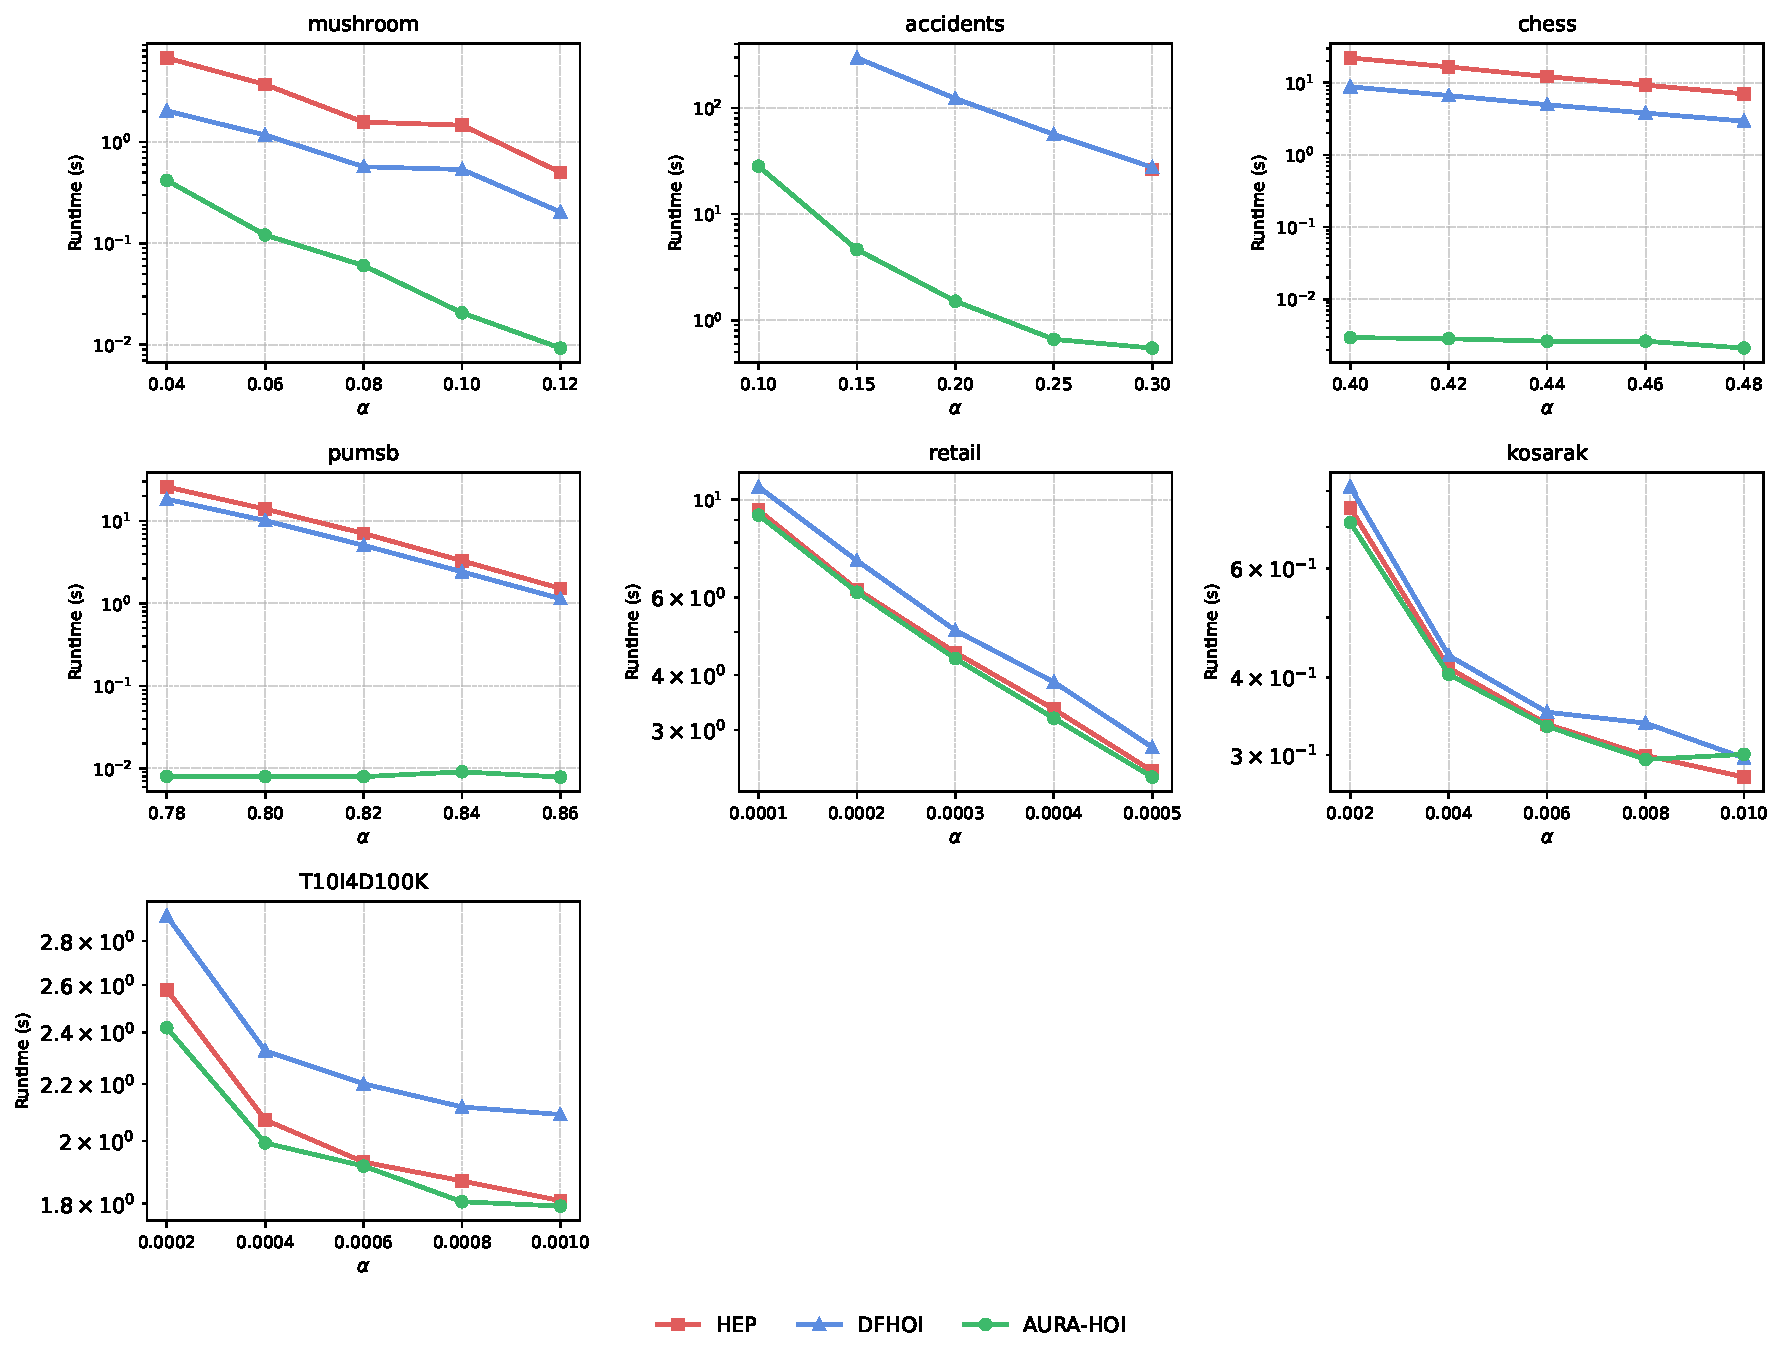
\includegraphics[width=\linewidth]{figures/runtime.pdf}
\caption{Runtime (seconds, logarithmic scale) as a function of the threshold $\alpha$. Missing points exceeded the memory limit.}\label{fig:runtime}
\end{figure}

\begin{figure}[t]
\centering
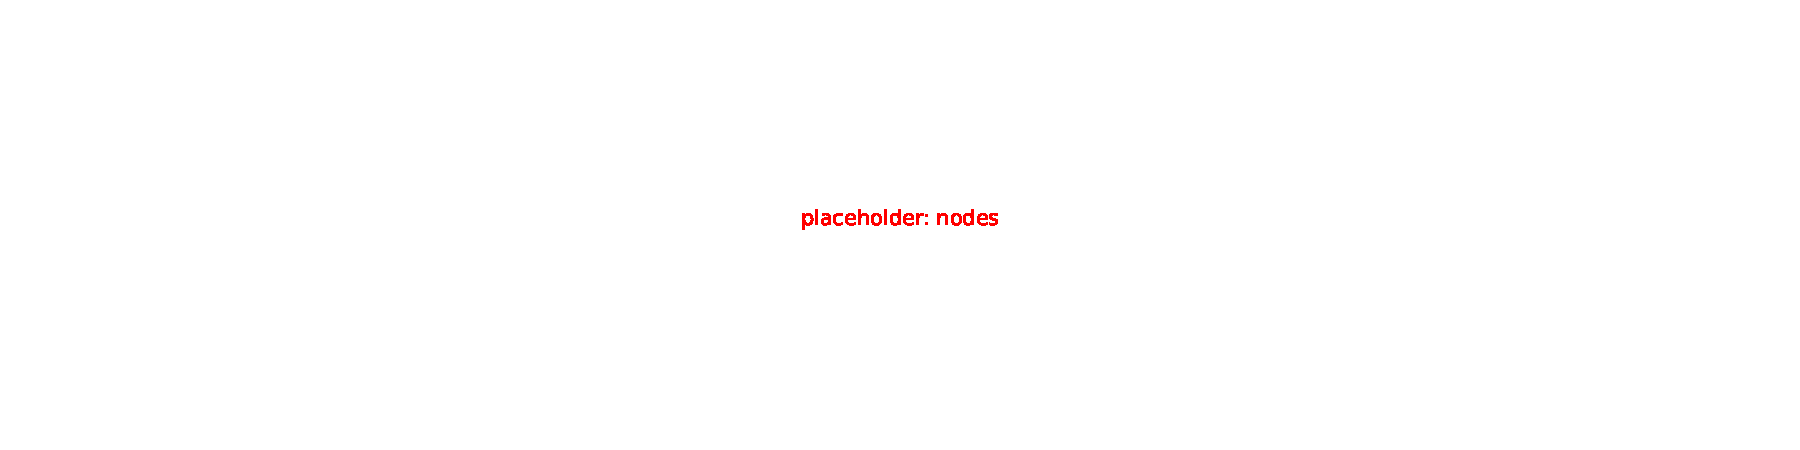
\includegraphics[width=\linewidth]{figures/nodes.pdf}
\caption{Candidate intersections (logarithmic scale) as a function of the threshold $\alpha$.}\label{fig:nodes}
\end{figure}

\pending{Runtime discussion: to be written from the final results.}

\subsection{Memory}\label{sec:exp-memory}

\pending{Memory discussion: to be written from the final results.}

\begin{figure}[t]
\centering
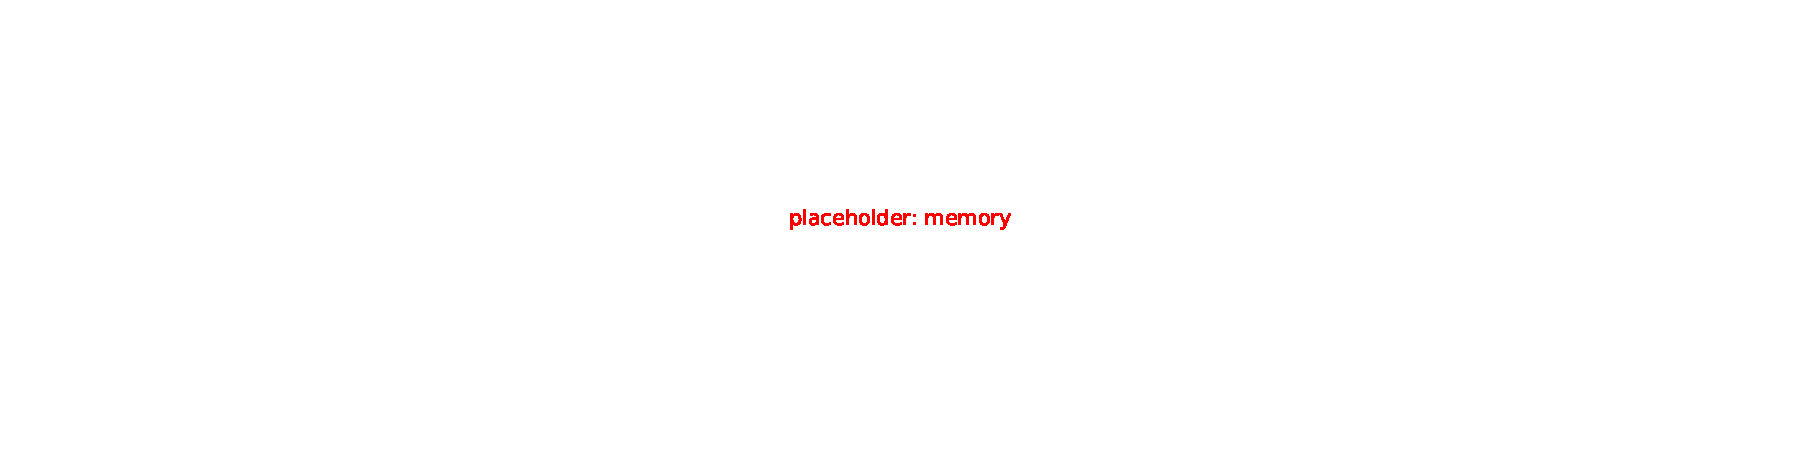
\includegraphics[width=\linewidth]{figures/memory.pdf}
\caption{Peak memory attributable to mining (MB, logarithmic scale).}\label{fig:memory}
\end{figure}

\subsection{Ablation study}\label{sec:exp-ablation}

To measure the contribution of each component, we disabled them one at a time: \emph{no tail cap} uses the transaction-length bound \eqref{eq:ubo} instead of $\Ucap_K$ in rule R2; \emph{no class bound} removes rule R3; \emph{no residual} does both, so that only transaction lengths are used, as in DFHOI; and \emph{no arena} allocates every TID-list on the heap. Table~\ref{tab:ablation} reports runtime and candidate intersections.

\begin{table}[t]
\caption{Ablation study: runtime in seconds and, in parentheses, candidate intersections. ML: memory limit exceeded.}\label{tab:ablation}
\centering
\footnotesize
\begin{tabular}{@{}lrlllll@{}}
\toprule
Dataset & $\alpha$ & Full & No tail cap & No class bound & No residual & No arena \\
\midrule
\inputrows{tables/ablation.tex}
\botrule
\end{tabular}
\end{table}

\pending{Ablation discussion: to be written from the final results.}

\subsection{Scalability}\label{sec:exp-scal}

\pending{Scalability discussion: to be written from the final results.}

\begin{figure}[t]
\centering
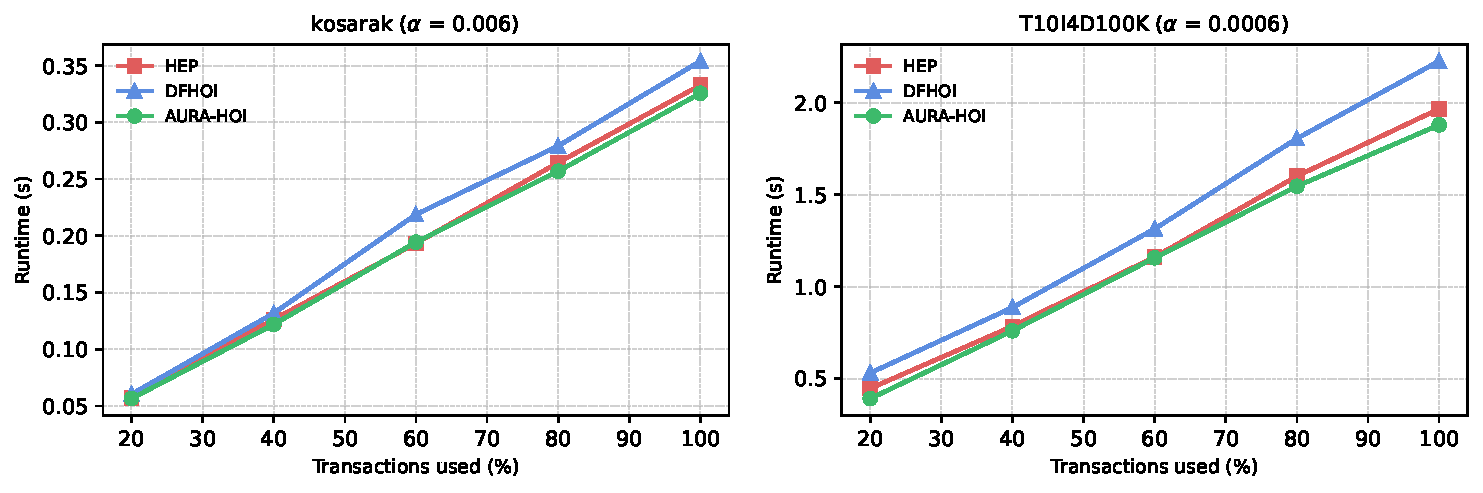
\includegraphics[width=\linewidth]{figures/scalability.pdf}
\caption{Runtime on growing prefixes of the database at a fixed threshold.}\label{fig:scal}
\end{figure}

\subsection{Limitations}\label{sec:exp-limits}

\pending{Limitations (pumsb, sparse data): to be written from the final results.}

%%%%%%%%%%%%%%%%%%%%%%%%%%%%%%%%%%%%%%%%%%%%%%%%%%%%%%%%%%%%%%%%%%%%%%%%%%%%%%%%
\section{Conclusion}\label{sec:concl}

\pending{Conclusion: to be written from the final results.}

\backmatter

\bmhead{Acknowledgements}
Not applicable.

\section*{Declarations}

\begin{itemize}
\item \textbf{Funding:} Funding not applicable. This research received no specific grant from any funding agency in the public, commercial, or not-for-profit sectors.
\item \textbf{Competing interests:} The author declares no competing interests.
\item \textbf{Ethics approval and consent to participate:} Not applicable.
\item \textbf{Consent for publication:} Not applicable.
\item \textbf{Data availability:} All datasets are publicly available from the FIMI repository \cite{fimi2004repository} and the SPMF library \cite{spmfdatasets}.
\item \textbf{Materials availability:} Not applicable.
\item \textbf{Code availability:} The source code of the three implementations and the scripts that reproduce every experiment are available from the corresponding author on reasonable request.
\item \textbf{Author contribution:} Q.~Van conceived the method, proved the results, implemented the algorithms, performed the experiments and wrote the manuscript.
\end{itemize}

\begin{appendices}
\section{Results for every configuration}\label{app:full}

\begin{footnotesize}
\setlength{\tabcolsep}{3pt}
\begin{longtable}{@{}lrrrrrrrrrr@{}}
\caption{Runtime (s; median of the repetitions; fastest in bold), candidate intersections and peak memory attributable to mining (MB) for every configuration. ML: memory limit exceeded; ML$^*$: not run because the same algorithm exceeded the memory limit at a larger threshold.}\label{tab:full}\\
\toprule
 & & & \multicolumn{3}{c}{Runtime (s)} & \multicolumn{2}{c}{Intersections} & \multicolumn{3}{c}{Memory (MB)} \\
\cmidrule{4-6}\cmidrule{7-8}\cmidrule{9-11}
Dataset & $\alpha$ & HOIs & HEP & DFHOI & \AURA{} & DFHOI & \AURA{} & HEP & DFHOI & \AURA{} \\
\midrule
\endfirsthead
\toprule
Dataset & $\alpha$ & HOIs & HEP & DFHOI & \AURA{} & DFHOI & \AURA{} & HEP & DFHOI & \AURA{} \\
\midrule
\endhead
\inputrows{tables/full.tex}
\botrule
\end{longtable}
\end{footnotesize}
\end{appendices}

\bibliography{aura_hoi}

\end{document}
